\let\negmedspace\undefined
\let\negthickspace\undefined
\documentclass[journal]{IEEEtran}
\usepackage[a5paper, margin=10mm, onecolumn]{geometry}
%\usepackage{lmodern} % Ensure lmodern is loaded for pdflatex
\usepackage{tfrupee} % Include tfrupee package

\setlength{\headheight}{1cm} % Set the height of the header box
\setlength{\headsep}{0mm}     % Set the distance between the header box and the top of the text

\usepackage{gvv-book}
\usepackage{gvv}
\usepackage{cite}
\usepackage{amsmath,amssymb,amsfonts,amsthm}
\usepackage{algorithmic}
\usepackage{graphicx}
\usepackage{textcomp}
\usepackage{xcolor}
\usepackage{txfonts}
\usepackage{listings}
\usepackage{enumitem}
\usepackage{mathtools}
\usepackage{gensymb}
\usepackage{comment}
\usepackage[breaklinks=true]{hyperref}
\usepackage{tkz-euclide} 
\usepackage{listings}
\usepackage{gvv}                                        
\def\inputGnumericTable{}                                 
\usepackage[latin1]{inputenc}                                
\usepackage{color}                                            
\usepackage{array}                                            
\usepackage{longtable}                                       
\usepackage{calc}                                             
\usepackage{multirow}                                         
\usepackage{hhline}                                           
\usepackage{ifthen}                                           
\usepackage{lscape}
\usepackage{circuitikz}
\tikzstyle{block} = [rectangle, draw, fill=blue!20, 
    text width=4em, text centered, rounded corners, minimum height=3em]
\tikzstyle{sum} = [draw, fill=blue!10, circle, minimum size=1cm, node distance=1.5cm]
\tikzstyle{input} = [coordinate]
\tikzstyle{output} = [coordinate]


\begin{document}

\bibliographystyle{IEEEtran}
\vspace{3cm}

\title{5.9.3}
\author{EE25BTECH11049 - Sai Krishna Bakki}
 \maketitle
\vspace{-3em}
% \newpage
% \bigskip
{\let\newpage\relax\maketitle}

\renewcommand{\thefigure}{\theenumi}
\renewcommand{\thetable}{\theenumi}
\setlength{\intextsep}{10pt} % Space between text and floats


\numberwithin{equation}{enumi}
\numberwithin{figure}{enumi}
\renewcommand{\thetable}{\theenumi}

\textbf{Question:}\\
Two schools \textbf{P} and \textbf{Q} decided to award prizes to their students for two games of Hockey \rupee~x per students and cricket \rupee~y per student. School \textbf{P} decided to award a total of \rupee~9,500 for the two games to 5 and 4 students respectively; while school \textbf{Q} decided to award \rupee~7,370 for the two games to 4 and 3 students respectively. Based on the given information, answer the following questions :
\begin{enumerate}
    \item Represent the following information algebraically (in terms of x and y).
    \item \begin{enumerate}
        \item What is the prize amount for hockey ?
        \item Prize amount on which game is more and by how much ?
    \end{enumerate}
    \item What will be the total prize amount if there are 2 students each from two games ?
\end{enumerate}
\textbf{Solution:}\\
Given\\
For Schools \textbf{P} and \textbf{Q}:\\
\begin{align}
5x + 4y = 9500 \\
4x + 3y=7370\\
\implies
\myvec{5&4\\4&3}\myvec{x\\y}=\myvec{9500\\7370}
\end{align}
\begin{align}
    \augvec{2}{1}{5&4&9500\\4&3&7370}\xleftrightarrow{R_1\rightarrow R_1-R_2}\augvec{2}{1}{1&1&2130\\4&3&7370}\\
    \augvec{2}{1}{1&1&2130\\4&3&7370}\xleftrightarrow{R_2\rightarrow R_2-4R_2}\augvec{2}{1}{1&1&2130\\0&-1&-1150}\\
    \augvec{2}{1}{1&1&2130\\0&-1&-1150}\xleftrightarrow{R_1\rightarrow R_1+R_2}\augvec{2}{1}{1&0&980\\0&-1&-1150}\\
    \augvec{2}{1}{1&0&980\\0&-1&-1150}\xleftrightarrow{R_2\rightarrow -R_2}\augvec{2}{1}{1&0&980\\0&1&1150}\\
    \myvec{x\\y}=\myvec{980\\1150}
\end{align}
$\therefore$ The prize amount for Hockey(x) and Cricket(y) respectively are \rupee~980 and \rupee~1150.
The Prize amount of Cricket is more than Hockey by a difference of \rupee~170.
\begin{align}
    \text{Total amount}= \myvec{2&2}\myvec{x\\y}\\
    \text{Total amount}= \myvec{2&2}\myvec{980\\1150}\\
    \text{Total amount}=1960+2300 \notag\\
    =4260
\end{align}
$\therefore$ The total prize amount if there are 2 students each from two games is \rupee~4260.
    \begin{figure}[H]
    \centering
    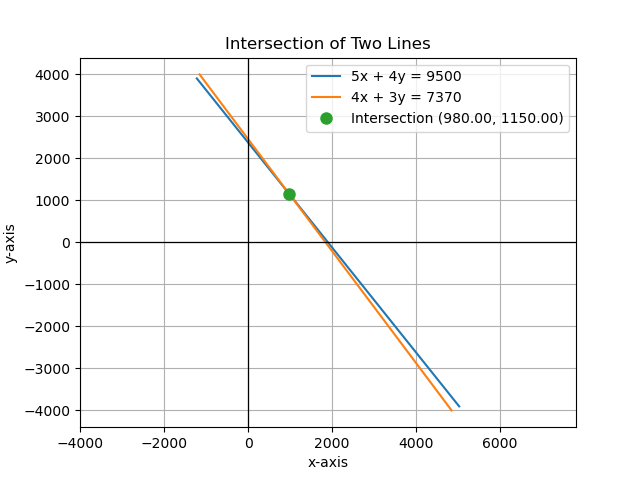
\includegraphics[width=0.7\columnwidth]{figs/Figure_1.png}
    \label{fig:placeholder}
    \caption{1}
\end{figure}
\end{document}